\section{Metodología}

Para el desarrollo de este proyecto se utilizará la metodología ágil. La razón por la que decidió utilizar esta estrategia de desarrollo sobre otras metodologías lineales (como la metodología de casacada) es que soporta el trabajo simultáneo de varias etapas del desarrollo de software. De esta manera, se puede diseñar, desarrollar y probar en pequeños ciclos iterativos hasta que la funcionalidad satisfaga los objetivos definidos \cite{what_is_agile_meth}. Este proyecto se dividirá en los siguientes puntos:

\begin{itemize}
	
	\item La red inalámbrica de sensores que se utilizará para monitorear el clima del invernadero tendrá una topología de estrella, donde la computadora central será un \textit{raspberry pi}. Esta será el punto de acceso, servidor DHCP y servidor DNS de los nodos que conformen la red inalámbrica. Se utilizará \textit{Hologram Nova} para acceder a internet a través de una red celular. Esta computadora será la única con acceso a internet.

	Los nodos de la red se comunicarán con la computadora central a través de HTTPS, utilizando JSON como formato para el intercambio de datos. Esto será posible gracias a que esta alojará un API REST que recibirá los datos obtenidos por cada nodo. En la Figura \ref{fig:coms_nodos_raspberry} se puede apreciar un diagrama general de la red inalámbrica de sensores.

	\begin{figure}[!ht]
		\centering
		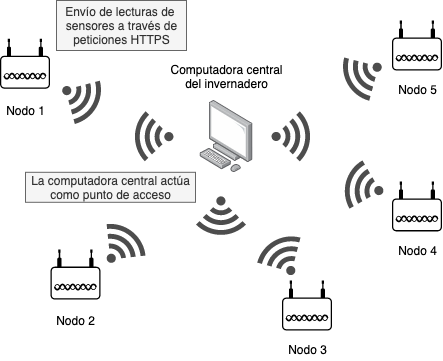
\includegraphics[width=.60\linewidth]{imagenes/diagramas/comunicacion_nodos_raspberry.png}
		\caption{Comunicación entre nodos de la red inalámbrica y la computadora central.}
		\label{fig:coms_nodos_raspberry}
	\end{figure}

	Se utilizará un microcontrolador Node MCU-ESP826 en cada nodo para sensar los sensores y enviar los datos a la computadora central. Este cuenta con pines para lecturas digitales y análogas. Además, este microcontrolador ofrece la ventaja de poder utilizarlo en una red de malla con hasta 100 metros de distancia entre nodos \cite{nodemcu_mesh}, lo cual es importante tener en consideración para determinar la escalabilidad del proyecto. Otra ventaja que ofrece es su modo de ahorro de energía, el cual permite que el dispositivo entre a un modo de `sueño profundo' donde su consumo de energía es mínimo \cite{nodemcu_datasheet}. 

	Los sensores que se utilizarán para hacer las mediciones son los siguientes:
	\begin{itemize}
		\item \textbf{DHT22}: Sensor de temperatura y humedad del ambiente. Envía una señal digital a través del pin de datos. Utiliza de 3 a 5 volts de poder. Tiene un rango de 0-100\% para lecturas de humedad y de -40 a 80°C para las lecturas de temperatura \cite{dht22_product_page}.
		\item \textbf{VEML7700}: Sensor de iluminancia. Utiliza de 3.3 a 5 volts de poder. Detecta de 0 a 120,000 lux \cite{veml_product_page}. 
		\item \textbf{Sensor capacitivo de humedad del suelo}: Utiliza de 3.3 a 5 volts de poder. Envía señales análogas a través del pin AOUT \cite{capacitive_soil_sensor_specs}.
	\end{itemize}

	Existirán dos variantes de nodos (Figura \ref{fig:componentes_nodos_wsn}):
	\begin{itemize}
		\item \textbf{Variante 1}: Contará con los 3 sensores, DHT22, sensor de humedad del suelo y VEML 7700. Este estará ubicado a nivel del suelo donde se podrá utilizar efectivamente el sensor de humedad del suelo.
		\item \textbf{Variante 2}: Contará con 2 de los 3 sensores, DHT22 y VEML7700. Estará ubicado a una altura donde el cultivo no lo cubra para que los datos recabados por el sensor de iluminancia sean confiables.
	\end{itemize}

	\begin{figure}[!ht]
		\centering
		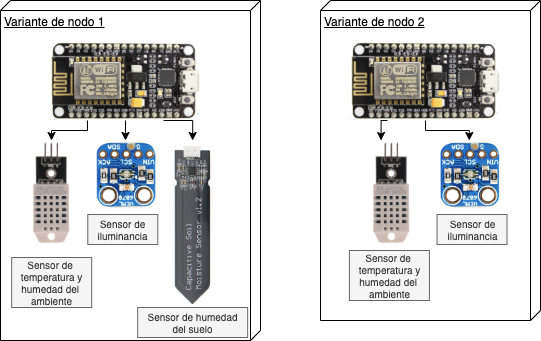
\includegraphics[width=.80\linewidth]{imagenes/diagramas/componentes_nodos_wsn.png}
		\caption{Variantes de nodos con sus componentes.}
		\label{fig:componentes_nodos_wsn}
	\end{figure}

	Después de que la computadora central reciba los datos enviados por los nodos de la red inalámbrica, estos se enviarán al servidor en la nube para que sean guardados en la base de datos. En la Figura \ref{fig:coms_vps_raspberry} se puede observar el diagrama de comunicación entre la computadora central y el servidor en la nube.

	\begin{figure}[!ht]
		\centering
		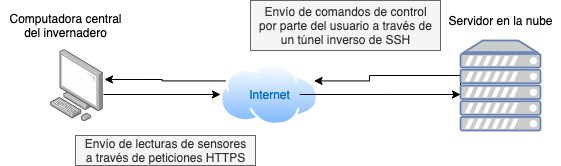
\includegraphics[width=.85\linewidth]{imagenes/diagramas/comunicacion_vps_raspberry.png}
		\caption{Comunicación entre la computadora central del invernadero y el servidor en la nube.}
		\label{fig:coms_vps_raspberry}
	\end{figure}

	El primer paso en el desarrollo de la red inalámbrica de sensores será la configuración de la computadora central para que tenga acceso a internet a través la red celular. Después, esta computadora se configurará como punto de acceso, servidor DNS y servidor DHCP.

	Posteriormente, se desarrollarán ambas variantes de nodos de la red y se conectarán al punto de acceso para comenzar a enviar los datos recabados por los sensores. Después, se harán pruebas del rango y de la estabilidad de la red antes de su implementación en el invernadero. Una vez pasadas las pruebas de estabilidad, se implementará la red inalámbrica de sensores en el invernadero, teniendo en cuenta el rango máximo entre nodos.

	\item Después se desarrollará un API REST para recibir los datos sensados por cada uno de los nodos que conforman la red inalámbrica de sensores y se enviarán al servidor en la nube a través de internet. Los datos recopilados por los nodos serán analizados al momento de ser recibidos para tomar decisiones de control sobre el clima y el riego del invernadero. Este API estará codificado en Python y se utilizará el \textit{framework} FastAPI.

	El API REST estará alojado dentro de la computadora central. Se utilizará NGINX como servidor web, este actuará como \textit{proxy} inverso y \textit{buffer} para el servidor de aplicación del API. Se utilizará PM2 como manejador del proceso principal del servidor de aplicación. Esto asegurará la disponibilidad de la aplicación. 
	
	\item Luego, se desarrollará un API REST en el servidor en la nube para recibir los datos recabados por la computadora central y, posteriormente, guardarlos en una instancia de MongoDB. Además, se encargará de la autenticación del cliente web para realizar las consultas de datos históricos y los comandos de control que se tengan que enviar a la computadora central del invernadero. Estará codificada en NodeJS gracias a las bibliotecas disponibles para la integración con la base de datos. Se probará el API durante el desarollo del mismo.

	El API REST estará alojado en un servidor privado virtual (VPS por sus siglas en inglés) de Digital Ocean. Se utilizará NGINX como servidor web, tanto para el API REST como para la aplicación web. Este actuará como un \textit{proxy} inverso para enviar las peticiones al servidor de la aplicación o a la aplicación web. Se utilizará el manejador de procesos PM2 para asegurar la disponibilidad del API REST al mantener el servidor de la aplicación siempre disponible. Los componentes que estarán alojados en el servidor en la nube se pueden apreciar en la Figura \ref{fig:componentes_vps}.

	\begin{figure}[!ht]
		\centering
		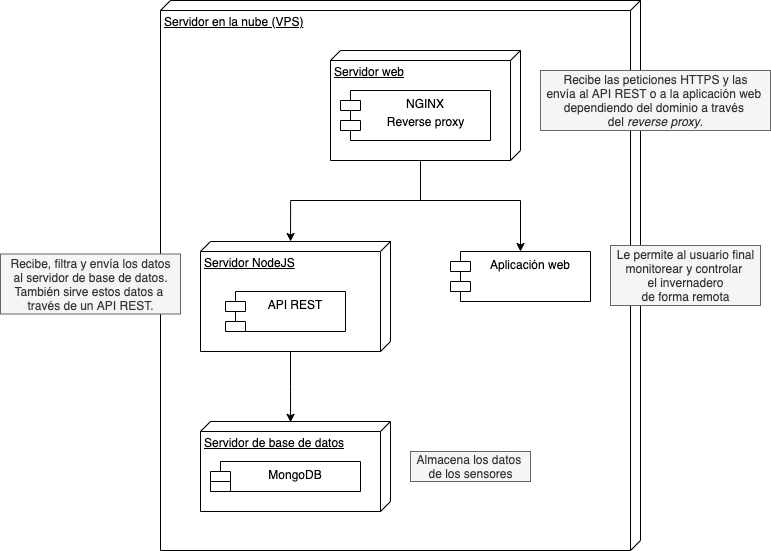
\includegraphics[width=.95\linewidth]{imagenes/diagramas/componentes_vps.png}
		\caption{Diagrama de componentes del servidor en la nube}
		\label{fig:componentes_vps}
	\end{figure}

	\item Posteriormente, se hará una investigación a fondo sobre la lógica difusa y su implementación en el área de control. Después, se diseñará un modelo para el invernadero en el cual se definirán las categorías para optimizar el control del riego y el clima. A partir del modelo, se buscará la mejor manera de hacer su implementación en la computadora central del invernadero.

	\item Finalmente, se harán maquetas de como serán las distintas interfaces del sistema. Se iterará sobre el diseño y la retroalimentación del usuario final. Se contarán con 2 vistas principales, la vista de autenticación y la vista donde se podrá realizar el control y monitoreo. El monitoreo se hará a través de la visualización de la información recabada por los sensores. Una vez que tanto el usuario como el desarrollador estén satisfechos con las interfaces, se procederá a la siguiente etapa.

	Se utilizará el \textit{framework} reactivo Vue.js como principal herramienta para el desarrollo de la interfaz. La comunicación con el servidor será a través de Javascript y XML asíncrono (AJAX por sus siglas en inglés) utilizando JSON como formato para el intercambio de datos. Al consumir el API REST que estará en el servidor en la nube se tendrá acceso a las mediciones históricas de los distintos sensores y se podrá hacer el control a través del mismo API. Se utilizará un \textit{JSON web token} (JWT) como \textit{token} de acceso al API. Este tendrá que ser enviado en todas las llamadas excepto en la que se utilice para iniciar sesión y obtener el primer \textit{token}. Las pruebas de esta aplicación web se harán durante el desarrollo de la misma.

	La aplicación estará alojada en el mismo servidor en la nube que la base de datos y el API REST con el que se recibirán y servirán los datos recopilados por los sensores. Se especifica la interacción con los demás componentes del servidor en la nube en la Figura \ref{fig:componentes_vps}.
\end{itemize}

% Modelo en cascada

% Análisis 
%     - Los parámetros que les importan a los agricultores los puedo sacar de unas encuestas
% Diseño
%     - Agregar imágenes de los sensores y agregar diagramas de la arquitectura que tendrá el sistema
% Implementación
%     - El microcontrolador se programará en Arduino, los datos se enviarán a través de HTTP
%     - En el rapberry puedo usar python (dependerá de las librerías de lógica difusa)
%     - En el servidor en la nube se utilizará un api en nodejs y se guardarán los datos en Mongo
%     - Para el front se va a utilizar Vuejs, el cual consultará los datos al API en la nube (se va a usar NGINX como servidor web)

%     - 


